% Chapter 1
\chapter{Literature Study} % Main chapter title

\label{Chapter2} % For referencing the chapter elsewhere, use \ref{Chapter1} 

\lhead{Chapter 2. \emph{Literature Study}} % This is for the header on each page - perhaps a shortened title

\setstretch{1}
%----------------------------------------------------------------------------------------

Business research question that will be addressed in this report concerns about detailed competitor analysis in the sector of movie recommendation engines. The task involves identification of competitors, investigation of the features provided by the competitors as compared to Vionel as a step forward in the business innovation process. The following paragraphs explains about background, need for recommendations, general problems of customer and the efforts of movie recommendation engine companies to solve problem of customers. It also explains about features supported by state of the art movie recommendation engines in current market.

\section {Background}

Every person spends a considerable amount of time in leisure activities by getting involved in recreational sports, surfing the web, watching television or other digital entertainment. With the advent of web and digital media technology, there has been an increase in time spent by  individuals on-line. It is also noticed that the trend of socializing through web has increased with the introduction of social media websites. As per a recent study, it has been observed that Americans, who do use computers for leisure spend a considerable amount of time per day watching digital content or playing on-line games and it is approximately of about hundred minutes per day \citep{time_spent_online}. Although the study did not mention about correlation of time spent on-line with variables such as time of the day, day of the week, age, occupation and other demographical information. It is clear that few aspects such as income and occupation plays an important role in influencing on-line presence of an individual. Nowadays, a larger chunk of those hundred minutes is spend in watching movies, television series and other videos available in social video sharing websites such as you-tube, vimeo etcetera.

Before computers took over the world, till the late of twentieth century people had access to media content, especially movies only through television and cinema theaters. Also the number of movies and other media content produced by year was considerably less as compared to current scenario the reason being due to introduction of state of the art technology. As per a recent statistical study by Statista website \citep{number_of_movies_per_year_online} the number of movies released per year has been consistently growing, this creates a favorable environment for businesses related to movies and digital entertainment. Movie franchises that are producing interesting movies for the viewers become the strongest complementer for our product. And also mobile gadgets companies, entertainment product manufacturers are assisting our service in an indirect way by increasing availability, ease of web access in various hand held mobile devices to get people engaged in digital media content for a longer duration of time. The information of time spent by an individual in a website is an actionable and interesting metric for the creators of the website. Naturally, given an average time spent by users, the owner of a website could estimate quality and popularity among the people on-line. Main objective of any website creator is not only to attract more number of unique visitors but also to engage them to spend more time by providing quality content. It also enables users to publish content into the web, on the other hand users have an access to large volumes of information at their convenience. 

\section{Need for movie recommendations}

The problem with availability of more information at one place is that it could create a sense of confusion for the users to decide and chose suitable information from the available content especially if the options are equally good. The scenario in which users face ``what to watch ?'' barricade is a highly common occurrence in the case of on-demand content delivery services, especially in the case of movie on demand services, in which users can chose and watch a movie on-line in their leisure time. If the user has less clue about movie to watch, it can be really time consuming for the user to decide upon and chose a particular movie to watch. Also a lot of user's time can be spent on searching the on-line content to find the appropriate type of movie one likes to watch. When users are presented with more than million choices of movies to watch, as in the case of Netflix, the users have trouble in choosing a best content from the lot \citep{flicking_online}. In this scenario most of the users tend to switch to other websites or decide not to watch movie at that instance, which highly affect popularity of movie on demand service. In order to develop a better rapport with the users the companies have come up with an solution to assist its users in choosing movies to watch by providing suggestive list of movies. The software that provides suggestions is termed as a recommendation engine and in this particular case a movie recommendation engine. It solves the problem of user's confusion of choosing and deciding the movie content to watch.

\section{State of the art movie recommendation engine}
\label{State of the art movie recommendation engine}
An ideal movie recommendation engine would present user with a personalized list of accurately predicted movies based on movie content, user's mood, taste and other behavioral aspects. It should be able to replace search engines for a movie recommender website, a user should be able to view the list of suggestive movies instead of manually searching for the movies one likes. The list of movies suggested by the recommender system should be accepted by the user at that instance, failure to do so might disappoint user and eventually one might loose trust over the generated results. A recent study about \acrshort{MRS} of Netflix shows that the predicted results include both blockbuster movies and movies that are less popular, this mix of suggestions motivates user to consume content from both categories \citep{Longtail_online}. Hence in a competitive market, there is a need for continuous innovation in recommender systems for predicting accurately movies needed by the customer at a given point in time. The accuracy and hence popularity of a movie recommendation system completely depends on the criteria used for generating predictive results. The predicted results can be solely based on features of a movie, its actors, directors, plot or it could be based on similarity between movies watched by user earlier and the current database of movies. The prediction list of movies should include movies that surprise the user, an example would be a list containing all action films except few of them belonging to other genre category which have similar directors, actors, speed of the movie, movie color tone and plot. It is also essential for an recommender engine to explain the reason for inclusion of such movies in the predicted results to convince users about its relevance in the list and there should be provision for the users to validate the generated results.  

A popular recommender engine should be able to generate diversified, relevant, personalized, customized, intriguing and dynamic results for each user. Nowadays, with the growth of digital social media a user can get information about latest movies, which is not the case for old movies that not popular and also movies that belong to a different geographic location. It is a good to have feature for recommender engine to be able to learn individual user's taste and to include these results in the recommendations. In a broader sense, recommender systems can be categorized into collaborative filter based, content based and hybrid recommender system \citep{Article_1}. It is observed that users generally choose movies with a similar kind of qualities, the system that learns about the user preferences over a period of time in a non intrusive way and uses the collected data as input to generate suggestions in future for the users is collaborative filtering based \acrshort{MRS}. Whereas content based \acrshort{MRS} predicts a list of movies to the user based on the similarity between preselected set of movies obtained from the user and database of movies. The last category of \acrshort{MRS} combines the idea of both content and collaborative based systems to refine the results and generate highly accurate results for the users. There is a shortcoming in case of recommendation engines referred to as cold start problem, which means that algorithm has very less information about a user to provide recommendations, this is the case for all new users. Hence availability of user data plays an important role in determining quality of recommendations.

In order to perform competitor analysis there is a need to understand features of a ideal \acrshort{MRS} in order to achieve comparatively better results from the competitors. Also a study of both technical and business strategies used by the competitors is required to learn from their mistakes and better our service.           

\section{About our competitors}

 After understanding needs of customer and market scenario for a product, next step is to know about competition. Competitors are the companies in similar domain or a similar product, a service offering owned by a company that poses threat to promotion of our product and competes to be popular among common customer segment. In essence, any entity that competes against our company by fighting for market share in the niche segment by providing better value to the customer for lower price or investment. The process of discovering competitors involves a lot of research using new papers, popular magazines in the domain, press releases, business articles and data available on-line. Filtering and shortlisting the competitors is crucial before performing a detailed competitor analysis by avoiding traps of considering a company with no relevance as a competitor, on the other hand missing out a tough competitor could prove to be fatal for company's future. Competitor analysis provides decision makers with an valuable data about current scenario, which assists them to drive future of the company in right direction, to be beneficial for all stakeholders of a company. 
 
 All of our direct competitors have website as an interface with the end users. The Google page rank index of these websites provide a credible clue about the inbound traffic to these websites and the one with highest traffic is ranked as popular among its customers. Few of the major direct competitors for our product are as follows, Internet Movie Database (\acrshort{IMDB}), Fandango, Rotten tomatoes, Flixster, What to rent ?, Movie-lens, Criticker, Nanocrowd, Taste-kid, Jinni, a-good-movie-to-watch, suggest-me-a-movie. The graph displayed in figure \ref{fig: Popularity of competitors} provides information about popularity of our competitors in current market using data provided by \citep{popularity_online}. One more metric similar to popularity of recommender engines, is the duration of time spent by an average user in a website. Data collected by  provides information about average time spent by an user in popular recommendation engines, the graph is as displayed in figure \ref{fig: Time Spent by an average user} from data collected using Alexa \citep{Alexa_imdb} website. The comparison task involves measuring various metrics related to product or service offering and later analyzing collected data to arrive at conclusions. Analyzing various metrics regarding competitor recommender system will be useful in determining competitive position of offerings provided by Vion Labs. Determining competitive positioning in the current market is an essential task to be conducted in order to know relative position among competitors as perceived by the customers it serves \citep{Fleisher_411:2007:BCA:1408337}.  

 \begin{figure}[htbp]
	\centering
		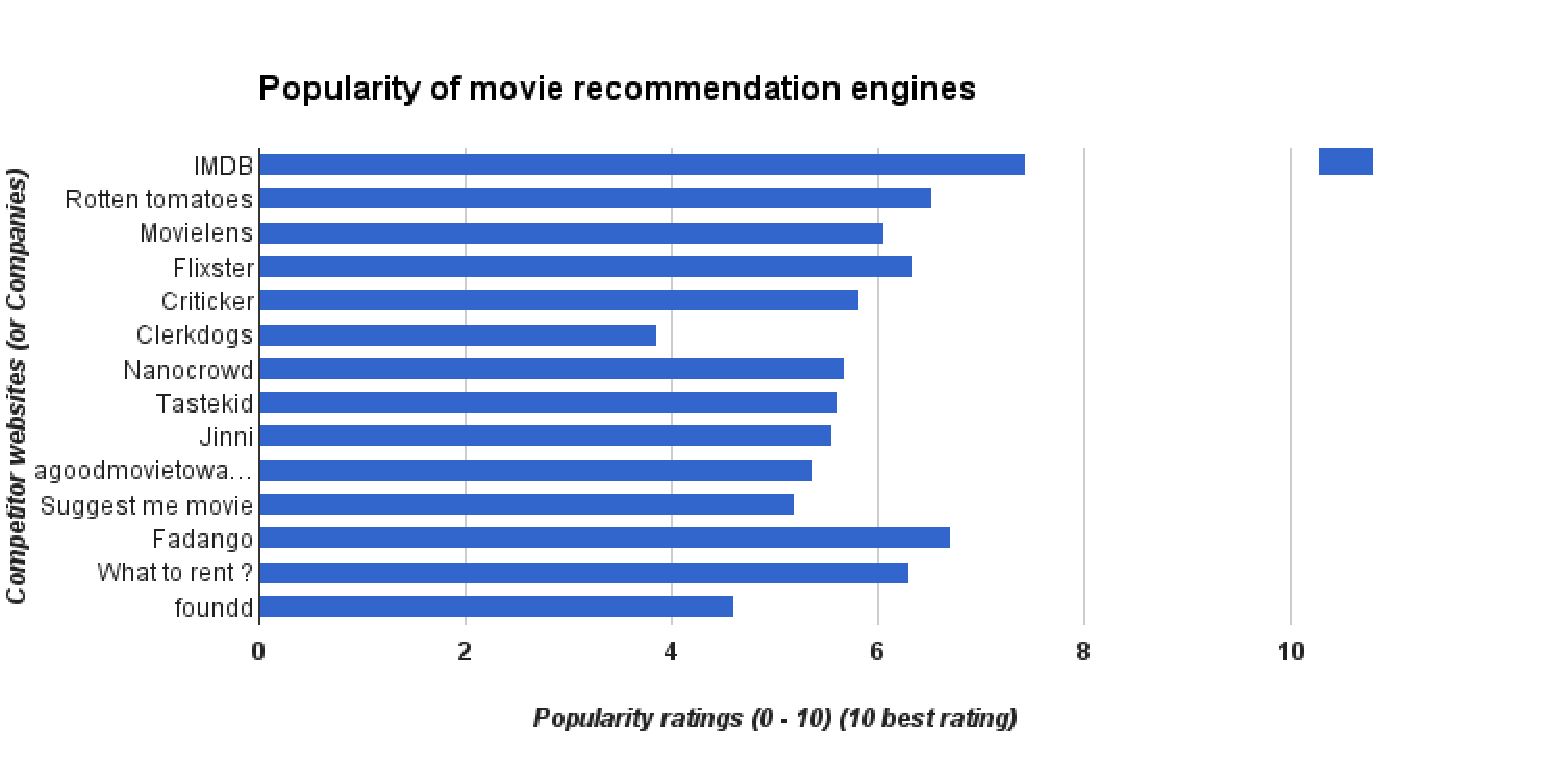
\includegraphics[scale=0.7]{Figures/competitor_popularity.pdf}
		%\rule{35em}{0.5pt}
	\caption[Graph: Popularity rating of competitors in the area of movie recommendation system]{Popularity of Vionel's competitors \citep{popularity_online}}
	\label{fig: Popularity of competitors}
 \end{figure}

 \begin{figure}[htbp]
	\centering
		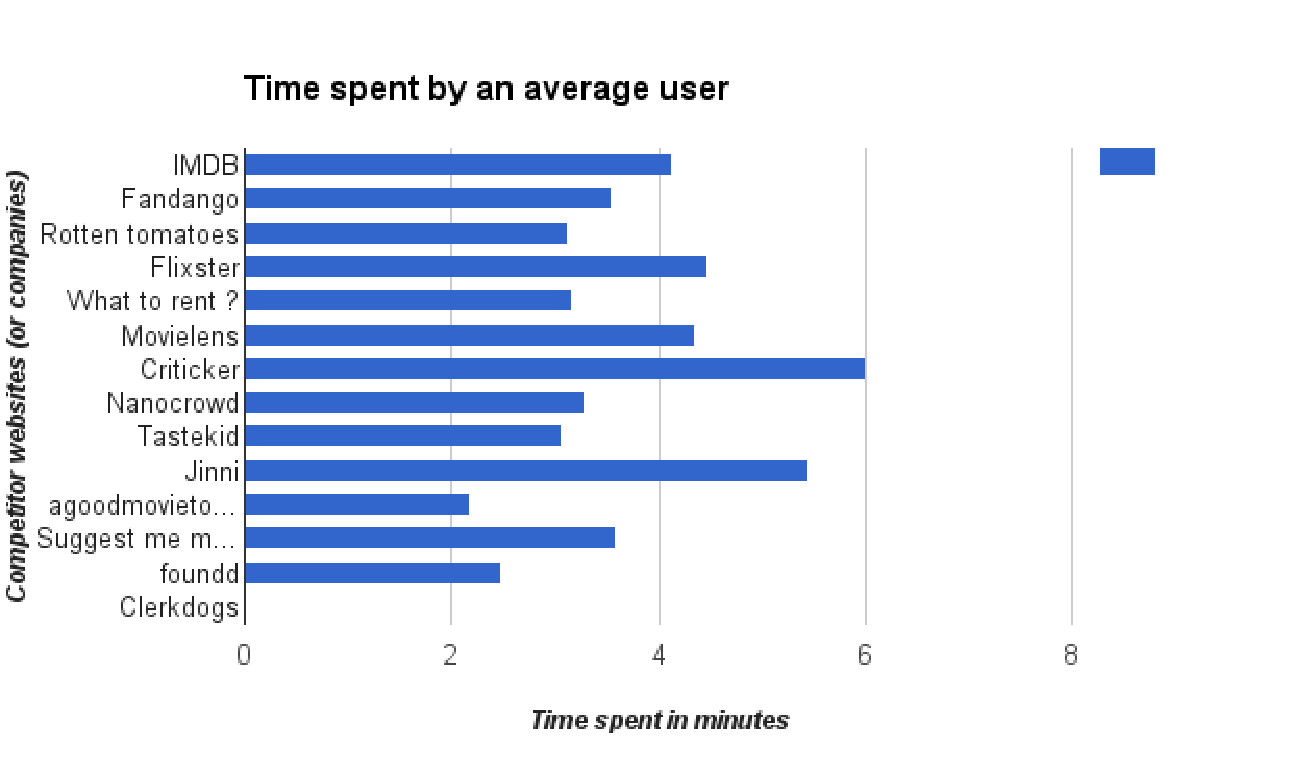
\includegraphics[scale=0.7]{Figures/fig_time_spent_each_recommender_site.pdf}
		%\rule{35em}{0.5pt}
	\caption[Graph: Average time spent by an user in popular movie recommendation websites]{Time spent by an average user in recommender websites\citep{Alexa_imdb}}
	\label{fig: Time Spent by an average user}
 \end{figure}

  
\section{Competitive advantage and technological differentiation}
\label{Competitive_advantage_tech_differentiation}
 For any company to beat the competitor to the market, there is a need for company to out think and produce a product that provides better value for customers at relatively same or less price. Technological development in a company's product which helps outranking competition in any form is essential to mark the presence of a firm in industry by gaining competitive advantage. In the domain of movie recommendation systems, technology plays an vital role in determining value provided to the customer and also helps in differentiating a product from its competitors. As described by Micheal Porter in \citep{Porter199806}, technological developments not only boosts the metric of differentiation from its competitors but it also increases firm's competitive advantage by influencing uniqueness of a product. Hence there is need for investments in research and development to improve recommendation algorithm. 

 Sustainable competitive advantage is achieved when a product of the company is able to provide a better value to the customer and continues to do so for a longer duration of time by creating barrier for other competitors to persuade its customers to switch the product. In the case of technology driven startups, sustainability is most of the times achieved by developing an highly innovative product or solution to the customers. As described by Byers and Nelson in \citep{ByersDorfNelson201401}, One more strategy of achieving sustainability is by collaborating with suppliers, complementers and other companies, which help in creating ample opportunities for development by building an sustained business ecosystem . The aim of collaborative strategies is to create powerful barriers for new entrants to enter into market segment. More about how Vion Labs is changing its strategy to achieve sustainable competitive advantage is described in section \ref{Changes_needed_to_face_the_challenge} of the report.  

\section{Information about Vionel's competitors}
 Since research question is about comparing features provided by \acrshort{MRS} in current market, five competitors are chosen to perform analysis and compare with Vionel. The following subsections provide overview of chosen competitors in the areas of unique features provided by them, revenue model used by them, the companies they have tied partnership with and also information about customer's view regarding recommendations offered. A critical aspect to study about competitors is to understand problems faced by them and the strategy used to overcome it. The following subsections capture all the related required information. Knowledge of unique features provided by competitors, helps us to rethink features provided by Vionel and improve our service. Inclusion of some features requires partnerships with other companies, hence partnership information of each competitor is collected during competitor survey. If some competitors use advertisement based revenue model, the web outlook feature of recommender system is greatly affected also, revenue model of competitors will help us to understand the underlying features in the framework. Finally, customers viewpoint about the service offered is summarized to compare it with Vionel and understand expectations of end users.     

 \subsection{Internet Movie Database Inc. (IMDB)}
  \label{IMDB_overview} 
  \subsubsection{Differentiating features}
    \label{IMDB_overview_DF}
    \acrshort{IMDB} has a wide collection of movies from all over the world, in fact it has highest collection of movie titles, related data items under one domain name. \acrshort{IMDB} supports both content based and collaborative based filtering to power its recommendation engine. Content based recommendations are as good as available content, \acrshort{IMDB} has around 180 million data items related to movies \citep{Press_imdb_online}. Currently the personalized recommendations are produced by collecting user's choices by monitoring on movies bookmarked by a user. Recommendations are not limited to popular movies, algorithm suggests movies from the non-popular category too. Recommendations are based on similar genre, tempo of the movie, similar actor and plot. It also cover movies from other languages, which have similarity to user's taste. One distinguishing feature is that it explains the reasons for suggesting a movie to the user, this creates a sense of assurance about quality of recommendations. \acrshort{IMDB} website outlook is easy to navigate, external advertisement free, provides information about new releases, suggestive movie lists from other users, actor and character information. It provides provision for users to navigate and search through movie content based on certain movie tags, for instance ``Movies based on Novels''.  

    \acrshort{IMDB} ratings are assigned to each movie content, based on its popularity among the users. A five star based rating information collection method from users is adopted to generate average ratings for a movie. Users are encouraged to cast votes for data items, including movie actors and movies.    
  \subsubsection{Revenue model}
    \label{IMDB_overview_RM}
    \acrshort{IMDB} uses cost per action (CPA) based revenue model in its website, the actions here refer to a user buying a movie using links provided in the website. With the recent acquisition of it by well know on-line retailer Amazon, it is clear that the trend is moving in the direction where retailers are buying out related publishing websites like \acrshort{IMDB} to improve their sales of movie DVDs, other movie related goodies \citep{How_I4_online}. Hence the core algorithm of \acrshort{IMDB} has modified to boost the sales of movie content providers like Amazon, also there is inclusion of ``buy from'' feature in website. Hence it can be observed that there is influence of revenue model to some of the features of a movie recommendation website. 
  \subsubsection{Information about partners}
    \label{IMDB_overview_IP}
    Partnerships with movie information content providers defines the quality of movie information that will be used for recommendations. Hence partnering with renowned movie production houses is essential for a company which has movie recommendation engine as product. \acrshort{IMDB} has partnerships with a good amount of movie production houses including other language movie production houses. Also partnership with on-line retailers and on-line movie on demand services is crucial for attracting more number of users. Some of the partners of \acrshort{IMDB} are MFP Munich Film Partners GmbH \& Company, Silver screen partners, Merced media partners, Armada partners, DirecTV and many more.   
  \subsubsection{Shortcomings and problems in recommendation algorithm }
    \label{IMDB_overview_SP}
    \acrshort{IMDB} requires the users to bookmark and rate at least twenty movies to be able to generate personalized movie recommendations. Most of the users tend not to bookmark and rate the movies that they like by searching for them manually. The quality of recommendations generated is as good as its input, hence \acrshort{IMDB} suffers from a cold start problem for each user. Currently, the recommendations are based on movie features like genre, popularity, actor similarity and character similarity, but there is room for including other features of movies to predict similarity between them for better prediction. 
     
  \subsection{Fandango Inc}
   \label{Fandango_overview}
   \subsubsection{Differentiating features}
   Fandango provides it users with a comprehensive search engine to find movies they like and also provides links to buy tickets if the movie is played in nearby cinema theaters. The search of movie theaters uses location information of the users. Movie reviews presented to users comprise of both critic based and registered user based reviews. Recommendation system uses both film critics based ratings and user based rating values for recommending movies to users. One innovative feature for benefit of parents is added, which alerts the users about allowed age for viewing a particular movie content. The five pointer rating meter is linked with abusive language, violence, scary scenes and other age restricted content for each movie. It also allows movie content such as posters, trailers, plot synopsis to be published in the website. Recommendations are content based, it uses movie genre, plot, actors and related data items to suggest movies to the user. A feature of allowing users to create alerts for a movie and get notified if there are movie tickets available in local theaters. 
  \subsubsection{Revenue model}
  \label{Fandango_overview_DF}
   Fandango has revenue model based on sales of movie tickets online. The recommendation engine suggests a newly released movie ,along with the link to buy tickets to watch movie in movie theaters. Unlike \acrshort{IMDB}, it has coupled a website publishing a movie content to movie theater franchises where movies can be watched in nearby locations to the user.    
  \subsubsection{Partners information}
  \label{Fandango_overview_IP}
   Fandango has partnered with Samsung TV to publish movie information in the form of trailers and also location based personalized links for users to buy movie ticket \citep{Fanda7_online}. The main partners for Fandango are movie theaters, some of the noticeable partners are AMC theaters, Premiere theaters, Georgia theater companies and many more.
  \subsubsection{Shortcomings and problems in recommendation algorithm } 
  \label{Fandango_overview_SP}
   The general image of Fandango among customers is that it is a website which sells movie tickets. Less number of people use it as a discovery platform to search for older or not so popular movies. Recommendation engine is biased towards movies that have tickets availability in theaters nearby to location of users.     

 \subsection{Jinni Inc}
  \label{Jinni_overview}
  \subsubsection{Differentiating features}
   Jinni provides its user with a personalized movie recommendations based on their entertainment personality, mood and taste. Unlike \acrshort{IMDB}, Jinni asks its users to chose short phrase related to type of movie to watch, such as ``Movies with scary storyline''. It contains around 40 -60 reliable tags for each movie title. It allows users to import ratings from other movie recommender websites, by reliving the pain of users to search for movies they like and re-rate them. Once the recommendation learns more about the user's taste, the recommendations generated are highly accurate and surprising. One more feature that is interesting for the users is to allow them to filter movies based on place, for instance if a user selects ``England'', all the movies related to this keyword are displayed to the users along with its trailers. Likewise, Jinni is planning to include speech based searches to enhance user engagement in website and on smart TVs \citep{Jinni0_online}. These features enable easy navigation for users with little or no computer knowledge. In the area of innovativeness, Jinni is found to be the best among the competitors.   
  \subsubsection{Revenue model}
  \label{Jinni_overview_RM}
    Jinni is in the path of creating an entertainment genome, which enables the algorithm to recognize a person's personality based on movies liked. The historical information about users watched content is used by Jinni to provided better entertainment recommendations for user in future. It provides services for smartTV and other over-the top content providers to provide personalized recommendations for users based on collected user data. For websites that host advertisements in the form of videos, Jinni provides application programming interfaces for generating personalized recommendations for its users.    
  \subsubsection{Partners information}
  \label{Jinni_overview_IP}
    Jinni recommendation api's are capable of predicting user behavior by using historical data collected. Any web related infrastructure where users are allowed to view videos, the api's are capable of generating personalized recommendations, hence some of the mobile application developing companies, web applications developers, smartTV providers, set up box providers have become partners with Jinni. The partners are Arris, seaChange, NDS and openTV. Hence Jinni's recommendation algorithm makes use of collected user data over a period of time to suggest movies in future with high accuracy. 
  \subsubsection{Shortcomings and problems in recommendation algorithm }
  \label{Jinni_overview_SP}
    Jinni's recommendation engine faces the problem of cold start for new user, for which algorithm has no history of collected data with it. Currently to solve the problem, soon after registration user needs to rate movies based on their tastes to enable algorithm to generate recommendations based on that list of movies. If a user is unwilling to do that there is a problem of user getting frustrated and leaving the service. 

  \subsection{A good movie to watch }
  \label{agoodmovietowatch_overview}
  \subsubsection{Differentiating features}
  \label{agoodmovietowatch_overview_DF}
    A good movie to watch provides its users with an on-line platform to discover popular movies based on their taste, also there is provision for discovering movies which are less known among the public. The website has a simple structure comprising of options for users to select tags for a movie to watch. The recommendations are content and ratings based, there is a high possibility that movies with less box office splash to come up in the list of recommended movies for the users. One of the interesting feature of this website is that it allows users to search for movies to be watched with a group of friends, family, crush or also movies to be watched alone. The innovativeness in the features provided by this website is good. It has links where to watch the liked movie content from, most of the times it is pointing to Netflix.
  \subsubsection{Shortcomings and problems in recommendation algorithm }
  \label{agoodmovietowatch_overview_SP}  
    The major shortcoming in this website is that the movie content starts from year 1982, it is a niche dataset with good quality movies in it.
    Database is built upon movies that have more than 6.7 movie ratings in \acrshort{IMDB} and more than 60 percent score in Rotten tomatoes \citep{Agoodmovietowatch_online}. Website lacks movie trailers that are essential for engaging movie enthusiasts to stay for more duration in  website.  

  \subsection{Foundd Inc}
  \label{Foundd_overview}   
  \subsubsection{Differentiating features}
  \label{Foundd_overview_DF}
    Foundd provides its user with a personalized recommendations based on their tastes and has a feature of collaborating with friends in social media websites. Provides a better user friendly, advertisement free web interface to browse through movie and TV series content. Mood based movie filtering is also a part of Foundd's content discovery platform. Users have to provide information about their entertainment personality to the recommender engine to start receiving movie suggestions. All activities on Foundd website are made socially available to friends in social media platforms. User privacy settings are allowed to change, there is provision for sharing rated movies history information with other users on Foundd. It has a continuously updated blog in web page to engage users to provide comments about overall service provided to them. It has feature of providing information about where to watch a movie, Netflix and other movie on demand website links are provided along with the displayed movie information.     
  \subsubsection{Shortcomings and problems in recommendation algorithm}
  \label{Foundd_overview_SP}
    Foundd also faces the problem of cold start that forces its users to manually search and rate at least ten movies they like in order to obtain good recommendations. Ratings based on film critics is missing, the ratings are only based on views of users on Foundd. Provision of filtering movies based on mood of a user is lacking. There is chances of creating an unreliable movie recommendation system, if the users are creating fallacy ratings for movies by deliberately trying to spoil rating system. Hence ratings from film critics also needs to be used to solve the problem of corrupt ratings. 
    
